\section{Contribuciones}

En esta sección se presentan las soluciones a las observaciones realizadas por
los sinodales durante la presentación del trabajo terminal 1.

\subsection{El juego}\label{juego}
El juego definida por la RAE es una actividad  recreativa o de competición sometida a reglas por el entretenimiento. Sin embargo más que ello es parte fundamental parael desarrollo y aprendizaje de cualquier individuao. Esta actividad contribuye a la maduración, potencia cognitiva, desarrollo emocional, vehículo emocional que contribuye para aprender nuevas habilidades y conceptos a través de su propia experiencia.

El juego refleja la percepción de sí mismos, de otras personas y del mundo que nos rodea. Por ello mismo cuenta con 5 grandes ventajas:
\begin{itemize}
	\item El juego otorga placer y felicidad.
	\item En el juego no se tiene miedo al error.
	\item Fomenta la creatividad.
	\item Práctica de creación de estrategias y colaboración.
	\item El juego es el aprendizaje natural de las personas.
\end{itemize}
	
\subsubsection{Teorías del aprendizaje}
Es el estudio del aprendizaje que concierne al proceso por el que ocurre según el libro "Teorías del aprendizaje" \cite{libroTeoApr}. Pues se necesita comprender algunas suposiciones generales de las teorías que sustentan el aprendizaje humano y de la forma en la que se construyen sus principios.

Las teorías más reconocidas sobre el aprendizaje son:
\begin{itemize}
	\item Gestalt: reestructuración perceptual.
	\item Piaget: Constructivismo genético.
	\item Vygotsky: Teoría sociocultural.
	\item Ausbel: Teoría del aprendizaje significativo.
	\item Bruner: Teoría cognitiva.
\end{itemize}

Aquella más cercana al juego para el trabajo a realizar es la teoría de Bruner. Pues el jugador que contempla es epistémico social, inserto en una cultura y estructurado por un lenguaje. La inteligencia esta relacionada con 3 etapas de desarrollo para conocer: ejecución, impresión o imagen y significado simbólico. La evaluación está enfocada al estudio integral de los procesos cognoscitivos y los cambios que se originan.


\subsubsection{Los videojuegos como medio de comunicación}
Los videojuegos gracias a sus características de alcance masivo y presentación interactiva al usuario, son considerados parte de las TIC (tecnologias de la información y comunicación). Estos son más atractivos e influyentes dado que se enfoca a el ocio y entretenimiento de las personas. 
Es así como podemos ver incluso a los videojuegos usados como publicidad, puede ser de manera implícita donde se muestre marcas o productos dentro de un escenario o situación del juego o explícita donde el mismo juego presenta a la marca mostrando sus cualidades y ventajas (en la mayoría de los casos de forma exagerada). Además podemos ahora combinar la expansión que nos da el internet junto con la diversión de un videojuego, posibilitando a los jugadores la capacidad de promover los productos que han probado y enseñarlo a los demás jugadores.


\subsubsection{Serious games}
Aquí podemos aprovechar la creación de un serious game, pues son los juegos digitales con una finalidad explícita para el aprendizaje más allá del entretenimiento sin ser pensados en la diversión. Tienen su interés en el desarrollo de las competencias, mediante actividades interactivas basadas en el juego.
Contribuyen al desarrollo de la coordinación ojo-mano, agudeza visual, reacción, atención múltiple, aptitud relacional, motivación, tolerancia a la frustración, toma de riesgos, resolución de problemas y toma de desiciones, así como la reflexión estratégica, la creatividad, cooperación y sentido de innovación {marqués, 2010, p.276}. Así mismo el jugador mejora el desempeño y se adentra a la experimentación, dada una situación simulada en la realidad virtual sin tener que enfrentar los riesgos de la realidad. 

La gamificación y game-based learning son herramientas que persiguen el mismo objetivo de atraer y hacer practicar experiencias para memorizar y retener contenidos. Pueden usarse como ayuda para crear un serious game.

La gamificación es el uso de elementos de juego y técnicas de diseño para potenciar la motivación y compromiso de los jugadores. Mientras game-based learning se refiere al área cognitiva y apariencia donde debe crearse una experiencia de aprendizaje positiva.

En el siguiente cuadro\cite{gabale} establecemos las diferencias más destacadas en ambás técnicas.

\begin{table}[htbp]
	\centering
	\caption{Diferencias entre gamificación y game-based learning}
	\label{gabale}
	\begin{tabular}{ll}
		Gamificación                                                        & Game-based learning                                                         \\
		Incluir los mecanismos de los juegos a situaciones de aprendizaje   & Usar los juegos para crear una experiencia de aprendizaje                   \\
		Existen como motivadores puntos de experiencia, logros e incentivos & La experiencia va dirigida al pensamiento crítico y resolución de problemas \\
		Enriquece la ambientación y simulación del aprendizaje              & Ambientación y simulación controlada a solo eventos positivos              
	\end{tabular}
\end{table}

\subsubsection{Motivos para jugar}
El área de interés para el desarrollo del trabajo es la gamificación, para ello la parte importante a conocer son los diferentes motivantes que tiene una persona al jugar.

Para determinar el perfil motivacional se tomará la "rueda de motivos"\ref{fig:rm} definida por Valderrama\cite{valde}, donde se define motivos de aproximación; aquellas personas sociales y buscan la convivencia y motivos de evitación; aquellas personas que prefieren la seguridad y estancia individual.
\begin{figure}
	\centering
	\caption{Rueda de motivos de Beatris Valderrama}
	\label{fig:rm}
	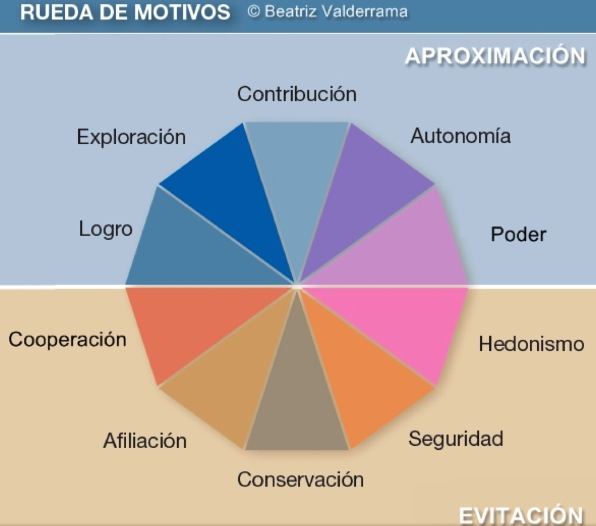
\includegraphics[width=0.5\textwidth]{imagenes\rueda-de-motivos}
\end{figure}

Es así como tenemos en contra partes diferentes motivos dependiendo del jugador obejtivo, que son la búsqueda de:
\begin{itemize}
	\item Logros o hedonismo
	\item Exploración o seguridad
	\item Contribución o conservación
	\item Autonomía o afiliación
	\item Poder o cooperación
\end{itemize}
 
\subsection{Modelo de negocios en un videojuego}\label{modeloNegocio}
Para sustentar un proyecto o producto económicamente se debe tener claro un modelo de negocios. En el mundo de los videojuegos no existe la excepción, pero también debe considerarse que existen formas muy diferentes de adquirir el ingreso.

Incluso el mismo juego puede estar involucrado en un ingreso directo del servicio.

\subsubsection{Mercado global}
Se reporta segun Newzoo \cite{newzoo2018} que 2.3 billones de jugadores en todo el mundo gastarán \$ 137.9 billones en juegos en 2018. Esto representa un aumento de + 13.3\% en comparación con el año anterior, o \$ 16.2 billones. Los ingresos por juegos digitales tomarán el 91\% del mercado global con \$ 125.3 mil millones, como podemos ver en la \ref{fig:merglo}
\begin{figure}
	\centering
	\caption{Mércado global al primer trimestre del año 2018 por Newzoo \cite{newzoo2018}}
	\label{fig:merglo}
	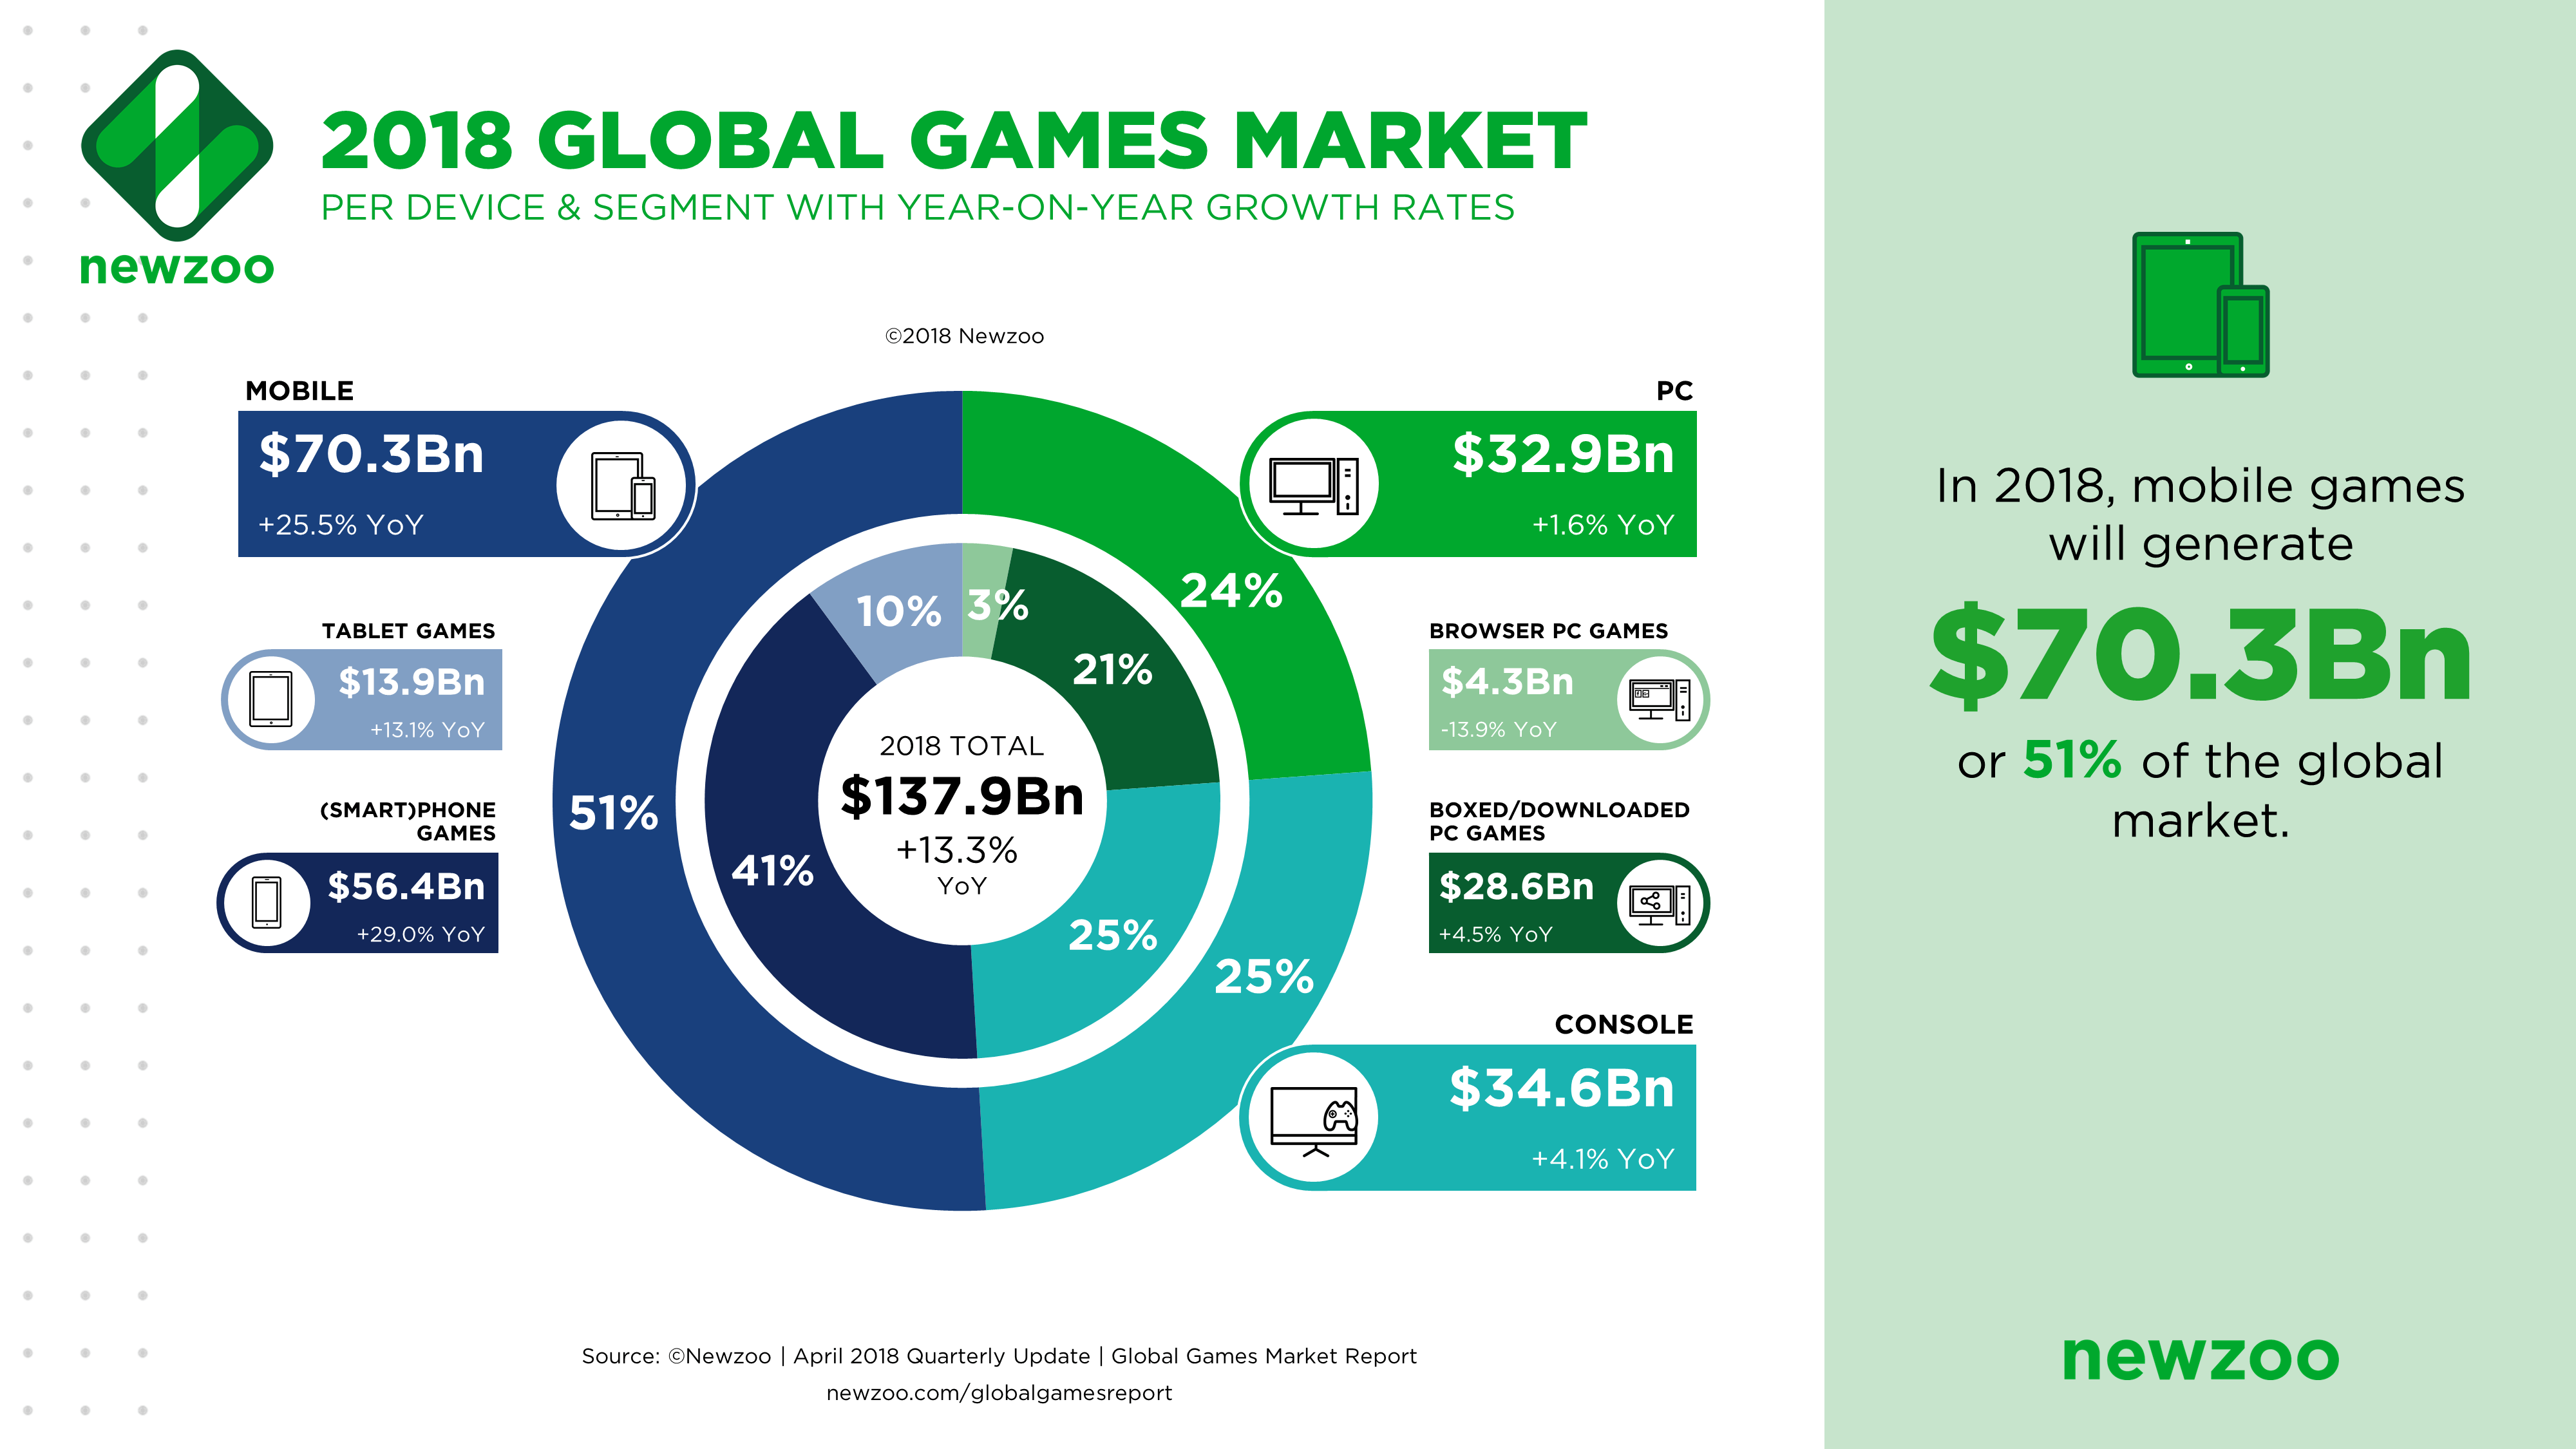
\includegraphics[width=0.5\textwidth]{02Antecedentes/contribucionesR/imagenes/merglo}
\end{figure}

Por primera vez, más de la mitad de todos los ingresos del juego provendrán del segmento móvil como vemos en la imagen{asdasd}. Los teléfonos inteligentes representarán el 80\% de esto, o \$ 56.4 mil millones, con el 20\% restante proveniente de tabletas.

\subsubsection{Salarios}
Para realizar un videojuego se necesita de diferentes profesiones para llevarlo a cabo.
En el siguiente cuadro \ref{tab:tablacostos} se mostrará la profesion y salario a recibir en la industria del videojuego en una empresa ya establecida al año 2014 segun la encuesta con una relación definida en experiencia.

% Please add the following required packages to your document preamble:
% \usepackage{multirow}
\begin{table}[htbp]
	\centering
\caption{Tabla de salarios dados en una empresa formal de videojuegos}
\label{tab:tablacostos}
\resizebox*{\linewidth}{!}{
	\begin{tabular}{|l|l|l|l|l|}
		\hline
		\textbf{Rama}                                                        & \textbf{Profesión}          & \textbf{Salario con -3años de exp.} & \textbf{Salario con 3-6años de exp.} & \textbf{Salario con +6años de exp.} \\ \hline
		\multirow{3}{*}{\textbf{Programadores e ingenieros}}                 & Programador                 & \$71,855 USD                        & \$79,877 USD                         & \$103,789 USD                       \\ \cline{2-5} 
		& Programador principal       &                                     & \$94,877 USD                         & \$116,151 USD                       \\ \cline{2-5} 
		& Director técnico            &                                     &                                      & \$135,781 USD                       \\ \hline
		\multirow{3}{*}{\textbf{Artistas y animadores}}                      & Animador                    & \$50,000 USD                        & \$55,547USD                          & \$82,230 USD                        \\ \cline{2-5} 
		& Artista principal           &                                     & \$71,029 USD                         & \$71,87576 USD                      \\ \cline{2-5} 
		& Director de arte            &                                     &                                      & \$110,000 USD                       \\ \hline
		\multicolumn{1}{|c|}{\multirow{2}{*}{\textbf{Diseñadores de juego}}} & Diseñador de juego          & \$53,000 USD                        & \$65,516 USD                         & \$77,768 USD                        \\ \cline{2-5} 
		\multicolumn{1}{|c|}{}                                               & Director creativo           &                                     & \$68,654 USD                         & \$101,944 USD                       \\ \hline
		\multicolumn{1}{|c|}{\multirow{3}{*}{\textbf{Productores}}}          & Productor asociado          &                                     & \$59,079 USD                         & \$61,912 USD                        \\ \cline{2-5} 
		\multicolumn{1}{|c|}{}                                               & Lider de proyecto           &                                     & \$73,500 USD                         & \$93,160 USD                        \\ \cline{2-5} 
		\multicolumn{1}{|c|}{}                                               & Productor ejecutivo         &                                     &                                      & \$126,833 USD                       \\ \hline
		\textbf{Profesional de audio}                                        & Director de sonido          &                                     &                                      & \$109,500 USD                       \\ \hline
		\multicolumn{1}{|c|}{\multirow{2}{*}{\textbf{Testers}}}              & Tester                      &                                     & \$38,833 USD                         &                                     \\ \cline{2-5} 
		\multicolumn{1}{|c|}{}                                               & Lider de control de calidad &                                     & \$60,417 USD                         & \$65,500 USD                        \\ \hline
		\multirow{3}{*}{\textbf{Negocios y administración}}                  & Marketing                   &                                     & \$73,500 USD                         &                                     \\ \cline{2-5} 
		& CEO                         &                                     &                                      & \$135,735 USD                       \\ \cline{2-5} 
		& Gerente ejecutivo           &                                     &                                      & \$156,731 USD                       \\ \hline
	\end{tabular}
}
\end{table}

\subsubsection{Presentación al cliente}
Un videojuego como cualquier software al momento de ser vendido al cliente puede encontrarse en dos presentaciones, una versión física o solo digital. En la siguiente tabla \ref{fiDi} se muestran las diferencias más destacables dadas por experiencia empresarial en el desarrollo por Velneo \cite{velneo2015}.

\begin{table}[htbp]
	\centering
	\caption{Tabla comparativa de un producto físico o digital por Velneo \cite{velneo2015}}
	\label{fiDi}
	\resizebox*{\linewidth}{!}{
\begin{tabular}{|l|l|l|}
	\hline
	\textbf{}                                             & \multicolumn{1}{c|}{\textbf{Físico}} & \multicolumn{1}{c|}{\textbf{Digital}} \\ \hline
	Coste de desarrollo                                   & sí                                   & sí                                    \\ \hline
	Coste de producción                                   & sí                                   & no                                    \\ \hline
	Coste de envío                                        & sí                                   & no                                    \\ \hline
	Riesgo de sobra/infra producir inventario             & sí                                   & no                                    \\ \hline
	Facturación por unidad vendida                        & mucho mayor                          & mucho menor                           \\ \hline
	Unidad vendida costea soporte                         & generalmente sí                      & imposible                             \\ \hline
	Porcentaje del precio de venta que percibe la empresa & 30\%-40\%                            & 70\%                                  \\ \hline
	Tiempo de cobro                                       & 90 días o más                        & 30 días                               \\ \hline
	Capacidad de llegar al público con marketing          & caro                                 & difícil                               \\ \hline
\end{tabular}
}
\end{table}

Aún así cabe mencionar que este es un aspecto general que involucra a cualquier software.

\subsubsection{Formas de ingreso}
Dentro de los videojuegos existen modelos de negocio que han dio cambiando a lo largo de los años y muchas de las veces depende del tipo del juego. Pero podemos definir las siguientes conforme lo visto y consumido en los últimos 5 años a la fecha del proyecto a presentar y con el apoyo de un artículo de la fundación UADE \cite{fundacionuade2014} en la tabla \ref{tablaMoneVJ}.

\begin{table}[htbp]
	\centering
	\caption{Tabla comparativa de ventajas y desventajas de modelos de negocios de videojuegos de autoría propia}
	\label{tablaMoneVJ}
	\resizebox*{\linewidth}{!}{
	\begin{tabular}{llll}
		Nombre       & Descripción                                                                                                               & Ventaja                                                                                                                                                                                                                                                                                                                  & Desventaja                                                                                                                                                                                                                                                                                                                                                                            \\
		Pay-to-play  & Se debe pagar contenido y uso del videojuego                                                                              & \begin{tabular}[c]{@{}l@{}}* Rápido retorno de inversión\\ \\ * Sin limitación de juego\\ \\ * Puede re-dirigirse a otro modelo en caso de fracaso \\ \\ * Puede ser un producto físico, por lo que puede cobrarse contenido extra\\ \\ * Complementa con compras in-game\end{tabular}                                   & \begin{tabular}[c]{@{}l@{}}* No compras por desconocimiento del juego (más en móviles)\\ \\ * Inversión grande por enfoque a consolas \\ \\ * Jugadores esperan contenido de entretenimiento de larga duración y calidad\\ \\ * No hay soporte o cambios en el juego\\ \\ * Si es un producto físico debe costearse la producción\\ \\ * Necesita publicidad\end{tabular}             \\
		Free-to-play & Ofrece gratis contenido y uso del videojuego en su totalidad, se monetiza con publicidad y compras in-game                & \begin{tabular}[c]{@{}l@{}}* Contacto con los jugadores más rápido\\ \\ * Preferente para móviles\\ \\ * Preferente para juegos de poca inversión (que quiera escalar)\\ \\ * Complementa con compras in-game\end{tabular}                                                                                               & \begin{tabular}[c]{@{}l@{}}* Depende de la cantidad de jugadores activos\\ \\ * Debe ser un juego con adicción para sustentarse\\ \\ * Debe ser un juego “infinito”\\ \\ * Requiere continuas actualizaciones si desea mantenerse\\ \\ * Debe darse al jugador contenido nuevo a jugar\end{tabular}                                                                                   \\
		Freemium     & Ofrece gratis el uso del videojuego pero no se accede a todo su contenido, establece jerarquización de tipos de jugadores & \begin{tabular}[c]{@{}l@{}}* Conveniente para demos (versión lite)\\ \\ * Oportunidad de dar a conocer el juego\\ \\ * Oportunidad de convencimiento al jugador\\ \\ * Contacto con los jugadores más rápido\\ \\ * Preferente para móviles\\ \\ * Viable aun sí existen pocos jugadores dispuestos a pagar\end{tabular} & \begin{tabular}[c]{@{}l@{}}* Debe crearse contenido de calidad por pago\\ \\ * Debe existir un control y registro de jugadores para su jerarquización\\ \\ * Usualmente el contenido extra debe ser descargado de internet (por lo que implicaría otros gastos y recursos)\\ \\ * Recomendable ser un juego “infinito”\\ \\ * A veces requiere continuas actualizaciones\end{tabular} \\
		Suscripción  & Se debe pagar el contenido y uso del videojuego pero con limitaciones.                                                    & \begin{tabular}[c]{@{}l@{}}* Es combinable con otros modelos como el freemium\\ \\ * Permite a los jugadores explorar el juego completo por cierto tiempo\\ \\ * Oportunidad de dar a conocer el juego\end{tabular}                                                                                                      & \begin{tabular}[c]{@{}l@{}}* Debe crearse contenido de calidad por pago\\ \\ * Recomendable ser un juego “infinito”\\ \\ * A veces requiere continuas actualizaciones\\ \\ * Debe darse al jugador contenido nuevo a jugar\\ \\ * Depende de la cantidad de jugadores activos\\ \\ * Debe ser un juego con adicción para sustentarse\end{tabular}         
	                           
	\end{tabular}
}
\end{table}



\subsubsection{Ingredientes de monetización}
Los modelos de negocio anteriores pueden ser combinables con otros "ingredientes" de monetización para acrecentarlos ingresos. 
\begin{itemize}
	\item Dinero virtual: Es el medio de intercambio que utiliza un videojuego para poder formalizar las compras dentro de él. A menudo se suele diferenciar el virtual currency (dinero virtual que se consigue por las propias mecánicas del juego y con abundancia) y el hard currency (dinero virtual premium que se consigue con dinero real o con acciones muy concretas y con mucha escasez).
	\item Bienes virtuales: Son objetos intangibles que son comprados e intercambiados que sólo tienen sentido dentro del juego, muchas veces estos son comprados con dinero virtual. 
	\item Publicidad y patrocinio: Anuncios o productos presentados en el juego para darse a conocer.
	\item Bonificaciones y servicios virtuales: Son aceleradores de juego o servicios que mejoran el desempeño o facilitan en el juego.
	\item DLC (downloadable content): Es un contenido de descarga digital exclusivo y adicional de un videojuego que se vende por separado y posterior al lanzamiento de este. Suele lanzarse para alargar la longevidad del videojuego y para aprovechar su éxito comercial. Su adquisición no tiene sentido sin tener antes el videojuego ya que es un producto complementario y dependiente a él.
\end{itemize}

%\subsection{Costo de hacer un videojuego}\label{costoVJ}

	
\subsubsection{Salarios}
Pararealizar un videojuego se necesita de diferentes profesiones parallevarlo a cabo.
En el siguiente cuadro se mostrará la profesion y salario a recibir en la industria del videojuego en una empresa ya establecida al año 2014 segun la encuesta ____ con una relación definida en experiencia.


\begin{table}[]
	\centering
	\caption{My caption}
	\label{my-label}
	\begin{tabular}{lllll}
		Rama                                                      & Profesión                   & Salario con \textless 3años de exp. & Salario con 3-6años de exp. & Salario con \textgreater 6años de exp. \\
		\multirow{3}{*}{Programadores e ingenieros}               & Programador                 & \$71,855 USD                        & \$79,877 USD                & \$103,789 USD                          \\
		& Programador principal       &                                     & \$94,877 USD                & \$116,151 USD                          \\
		& Director técnico            &                                     &                             & \$135,781 USD                          \\
		\multirow{3}{*}{Artistas y animadores}                    & Animador                    & \$50,000 USD                        & \$55,547USD                 & \$82,230 USD                           \\
		& Artista principal           &                                     & \$71,029 USD                & \$71,87576 USD                         \\
		& Director de arte            &                                     &                             & \$110,000 USD                          \\
		\multicolumn{1}{c}{\multirow{2}{*}{Diseñadores de juego}} & Diseñador de juego          & \$53,000 USD                        & \$65,516 USD                & \$77,768 USD                           \\
		\multicolumn{1}{c}{}                                      & Director creativo           &                                     & \$68,654 USD                & \$101,944 USD                          \\
		\multicolumn{1}{c}{\multirow{3}{*}{Productores}}          & Productor asociado          &                                     & \$59,079 USD                & \$61,912 USD                           \\
		\multicolumn{1}{c}{}                                      & Lider de proyecto           &                                     & \$73,500 USD                & \$93,160 USD                           \\
		\multicolumn{1}{c}{}                                      & Productor ejecutivo         &                                     &                             & \$126,833 USD                          \\
		Profesional de audio                                      & Director de sonido          &                                     &                             & \$109,500 USD                          \\
		\multicolumn{1}{c}{\multirow{2}{*}{Testers}}              & Tester                      &                                     & \$38,833 USD                &                                        \\
		\multicolumn{1}{c}{}                                      & Lider de control de calidad &                                     & \$60,417 USD                & \$65,500 USD                           \\
		\multirow{3}{*}{Negocios y administración}                & Marketing                   &                                     & \$73,500 USD                &                                        \\
		& CEO                         &                                     &                             & \$135,735 USD                          \\
		& Gerente ejecutivo           &                                     &                             & \$156,731 USD                         
	\end{tabular}
\end{table}

\subsection{Vicio en el videojuego}\label{vicioVJ}
Un videojuego se está convirtiendo en una adicción cuando la ansiedad se sobrepone al placer del juego y como síntoma se tiene la urgencia de jugar sin pensar en las consecuencias. El vicio se establece con cierta facilidad, ya que el juego ofrece un entorno de inmersión al combinar los aspectos interactivos e identificarse con el personaje o situación.

En la siguiente tabla se muestra las opiniones más comunes a favor y en contra de los videojuegos sin incluir mitos o falsedades, todas estás afirmaciones son demostrables o no han sido posible desmentirlas con hechos o pruebas concretas.
\begin{table}[htbp]
	\centering
	\caption{Opiniones comunes a favor y en contra de los videojuegos}
	\label{tab:tablaOpinión}
	\begin{tabular}{ll}
		A favor                                                            & En contra                          \\
		Entretienen                                                        & Provocan adicción                  \\
		Ejercitan la coordinación óculo-manual                             & Promueven conductas violentas      \\
		Estimulan la capacidad de lógica y reflexión                       & Aíslan socialmente                 \\
		Ayudan a concentrar la atención                                    & Limitan la imaginación             \\
		Son un potencial muy adecuado para distintas aplicaciones sociales & Restan tiempo de otras actividades
	\end{tabular}
\end{table}
\\[1pt]
	
\subsubsection{Síntomas de vicio}
A continuación se muestran síntomas identificables visualmente que ya representan una adicción al juego:
\begin{itemize}
	\item El jugador parece estar absorto al juego, sin atender cuando lo llaman.
	\item Siente demasiada tensión, incluso aprieta las mandíbulas cuando juega.
	\item No aparta la vista de la pantalla.
	\item Empieza a perder interés por otras actividades que practicaba.
	\item Trastornos del sueño.
	\item Distanciamiento de familia y amigos.
	\item No respeta los horarios estipulados.
\end{itemize}


\subsubsection{Carcaterísticas de un videojuego con potencial al vicio}
Los videojuegos (en especial los free-to-play) contienen características de vicio como: la necesidad de concluir “tareas incompletas”, síntomas de abstinencia y la posibilidad de jugarlo en todo momento. En este apartado solo mencionaremos algunas de ellas y almenos las más visibles en muchos videojuegos.

 \begin{itemize}
 	\item El efecto Zeigarnik: Se tiene incomodidad de las personas por tener “tareas incompletas”, en el caso de un videojuego se genera la necesidad por terminar el juego. El juego a su vez puede contemplar el nivel de porcentaje completado de un juego, provocando al jugador dicho síntoma haciéndolo jugar hasta su completado.
 	
 	\item Síntoma de abstinencia: En donde se priva o dificulta la posibilidad de realizar una actividad a una persona. En un juego tenemos como se establece turnos de juego, para recuperarlos se establece un límite de tiempo de espera. Usualmente estos tiempos de espera son de aproximadamente media hora o múltiplos de ella, pues psicológicamente este tiempo es lo que soporta una persona con una “tarea incompleta” en mente.
 	
 	\item La competencia: Que consiste en una disputa entre personas que aspiran a un mismo objetivo o a la superioridad en algo. Así, en un juego, ayudado en la mayoría de las veces por las redes sociales se puede compartir y comparar el avance entre los jugadores.
 	 \\[1pt]
 	
 \end{itemize}

\subsubsection{Causas del vicio ajenas al videojuego }
Entre los jóvenes entre 13 y 18 años especialmente existen muchas más causas para caer en el vicio de un videojuego, pueden ser factores psicológicos, emocionales, del entorno en el que se desarrollan y más. Incluso muchos de los factores siguientes encajan en otros tipos de adicciones.
\begin{itemize}
	\item Atención inexistente de los padres.
	\item No hay límites establecidos por la familia.
	\item Los valores no están asentados.
	\item Utilización de los videojuegos como "niñera".
	\item El joven no tiene sentido de pertenencia o no es aceptado en los grupos sociales que interactúa.
	\item Necesidad de escape de la realidad a un medio virtual.
	\item Establece mayor libertad expresión (o intenciones verdaderas) dentro del juego, ya sean positivas o negativas.
	\item Que la persona padezca alguna enfermedad que imposibilite realizar otras actividades .
	\item Trastornos psicológicos como depresión, impulsividad o ansiedad.
	\item Situación ante la solución de problemas y toma de decisiones.
	\item Falta de control emocional.
\end{itemize}

\subsubsection{Prevención del vicio}
Como toda adicción existen formas de prevenir llegar a ella.
Dadas las situaciones, causas, factores dentro del vicio del videojuego y con lectura de técnicas pedagógicas, las propuestas de solución se dan como sigue:

\begin{itemize}
	\item Establecer un horario de juego:
	\begin{itemize}
		\item Se puede poner una alarma que avise al jugador que ha estado jugando demasiado tiempo.
		\item Se puede programar a cierto tiempo jugado un bloqueo.
	\end{itemize}
	\item Complementariamente a la programación de un horario de juego, deberán establecerse qué actividades se llevarán a cabo en los momentos en los que no se va a jugar:
	\begin{itemize}
		\item Poder agregar al juego notas recordatorias de las actividades por hacer.
		\item Alarmas personalizadas dentro del juego.
	\end{itemize}
	\item Evitar los juegos online, al menos hasta que se tenga una organización del tiempo libre que impida dedicar mucho tiempo a dichos videojuegos.
	\begin{itemize}
		\item Evitar ser un juego online.
	\end{itemize}
	\item  No instalar la consola ni el ordenador en la habitación.
	\begin{itemize}
		\item El juego va a ser inaccesible a horas determinadas como la madrugada y noche.
	\end{itemize}
	\item Los padres deben conocer los videojuegos.
	\begin{itemize}
		\item Pedir forzosamente los correos de los tutores.
		\item Mandar mensajes a los tutores con un registro en resumen de lo que se está jugando.
		\item Habilitar una opción de bloqueo para los padres.
		\item Bloqueo automático e informe con estadística dependiendo de frecuencia de uso y tiempo de uso.
	\end{itemize}
\end{itemize}


\subsection{Modelo de datos}
La primera observación en atender fue el modelo de datos del juego, dicho modelo
de datos se realizó utilizando un modelo entidad relación de base de datos (Ver
Anexo \ref{Anexo:ModeloDatos}) ya que al modelarse de esta forma hace escalable
el juego si se deseara en algún futuro emplear una base de datos para mejorar
el almacenamiento de datos y el manejo de más usuarios para ofrecer un modo
online. El modelo de datos está basado en el modelo de clases y contiene
únicamente a las clases actoras. Toda entidad actora se define como una
especialización de una entidad base llamada GameObject, esta entidad está
definida por como su identificador y por otras entidades como GameObjectPosition,
Level, Tag, AnimationMachine, entre otros.

\subsection{Estrategias para combatir la adicción entre los usuarios}
La segunda observación sobre la que se trabajo fue como disminuir la adicción
del jugador al videojuego Yolotl. Esta observación dio lugar a una investigación
sobre la adicción a los videojuegos ya que antes de proponer alguna solución se
debía conocer cómo se definía, las causas y las consecuencias de la adicción al
videojuego. Al final de la investigación se pudieron formular tres posibles
soluciones para evitar la adicción del jugador; sin embargo, dado que este tópico
no estaba en la planeación original del proyecto y por el trabajo que
conlleva cada una de las soluciones se decidió únicamente describir las
soluciones y sus implicaciones sin desarrollar ninguna de las tres. A continuación,
se describen a manera de resumen las soluciones (nuevamente si se dese a
profundizar en la investigación realizada y las soluciones se puede consultar
el Anexo \ref{Anexo:AdiccJuga}):
    \begin{itemize}
        \item \textbf{Notificación de confirmación para continuar la partida.} Esta
        solución propone que el juego solicite la confirmación del usuario para
        continuar una vez que éste ha detectado que el jugador ha estado jugando
        durante un tiempo prolongado como una hora.
        \item \textbf{Control paterno.} El juego le envía un formulario al tutor del
        jugador por medio de un correo electrónico. En este formulario el tutor podrá
        decidir cuánto tiempo al día la aplicación podrá estar abierta.
        \item \textbf{Sistema de vidas.} El jugador tiene una cantidad de vidas
        limitadas. Cada vez que el jugador ingresa a un nivel o muere dentro de
        uno y reinicia la partida se gasta una vida. Para recuperar vidas el
        jugador deberá de esperar un determinado tiempo.
    \end{itemize}


